\chapter{Spatial Stochastic Simulations}


The spatial stochastic simulation capabilities in StochSS are based on PyURDME \cite{urdme}. PyURDME is a general software framework for modeling and simulation of stochastic reaction-diffusion processes on unstructured, tetrahedral (3D) and triangular (2D) meshes. The current core simulation algorithm is based on the mesoscopic reaction-diffusion master equation (RDME) model. The default solver is an efficient implementation of the next subvolume method (NSM) \cite{nsm}.

\section{Example: Annihilation of two species in a cylinder}
We will build a simple annihilation model based on an cylinder geometry. At each end of the cylinder, different chemicals will be produced. When they diffuse and meet at the center, they will annihilate each other.
\begin{enumerate}
\item Navigate to the main \textbf{Model editor}.
\item Add a new model. Select \textit{Population, spatial} in the dropdown menu.
 \item Click \textbf{Mesh} and select \textit{Cylinder}. The cylindrical mesh is divided into three subdomains which can be visualized with the controls below the wireframe view.
\item Add two species, $A$ and $B$, both with diffusion constant 1.
\item Click \textbf{Initial Condition}, select \textit{scatter}, and add 500 molecules of species $A$ in subdomain 1 and 500 molecules of species $B$ in subdomain 3. 
\item Add two parameters, $k0$ and $k1$, and set their values to 1 and 100, respectively.
\item Add three reactions:
\begin{align*}
\textrm{R1}:&\quad \emptyset\overset{k_1}{\rightarrow} A\\
\textrm{R2}:&\quad \emptyset\overset{k_1}{\rightarrow} B\\
\textrm{R3}:&\quad A+B\overset{k_0}{\rightarrow}\emptyset
\end{align*}
\item Reaction $R1$ should be restricted to subdomain 1 and reaction $R2$ to subdomain 3. Reaction $R3$ should be allowed throughout the whole domain.
\item The model is now complete and ready to be simulated.
\item Navigate to the \textbf{Simulation manager} page.
\item Select the spatial model you just created and click \textbf{Next}.
\item Setup the simulation parameters: name, time, data storage frequency, and number of realizations. 
\item You can specify a random seed for the random number generator under \textbf{Advanced Settings}.
\item Click \textbf{Run locally}.
\item In a few seconds you will be directed to the \textbf{Job Status} page where you can check the status of your simulation.
\item Once your simulation is complete, click \textbf{View results} to open the \textbf{Job summary} page, where you can visualize the diffusion of the two species over time within the cylindrical container and download the output files of the simulation.

\end{enumerate}

\section{Visualization (of Annhihilation of two species in a cylinder)}
Full three dimensional spatial stochastic simulations can be difficult to analyze. To simplify the process, StochSS has built in three different methods for visualization of spatial models.

\subsection{Surface Renderings with Domain Clipping}

By default, spatial stochastic simulations are rendered as shown in Figure \ref{surface}. These are surface renderings, but the simulations are volumetric. To see inside the volume, StochSS allows slicing the mesh in half along one axis with a plane and only rendering one of the resultant halves. This is shown in Figure \ref{clipx}

\begin{figure}[!ht]
  \centering
    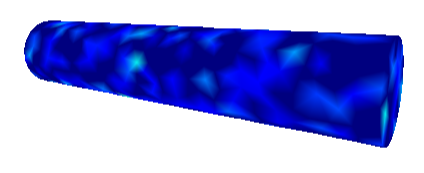
\includegraphics[width=0.5\textwidth]{surface}
  \caption{ Surface rendering of cylindrical domain. The actual stochastic simulation is run on the dual of the shown mesh, so the color at each node corresponds to the concentration in the corresponding voxel of the dual mesh. Colors are interpolated linearly between nodes. The color scale is not shown for brevity. }
  \label{surface}
\end{figure}

\begin{figure}[!ht]
  \centering
    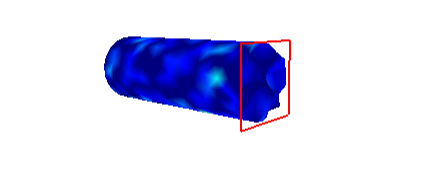
\includegraphics[width=0.5\textwidth]{clipx}
  \caption{ Surface rendering of cylindrical domain clipping along the X dimension. It is now possible to see concentrations of voxels inside the cylinder. }
  \label{clipx}
\end{figure}

\subsection{Colorized Wireframe Meshes}

The second rendering type is similar to the first, but instead of rendering surfaces only edges are rendered (see Figure \ref{wireframe}). The colorization is the same, it is just ideally easier to see inside the mesh. Similarly to the surface rendering the wireframe renderings can be clipped to get a clearer view of what is happening inside the volume. See Figure \ref{clipy} for a demonstration of clipping a mesh in the Y dimension.

\begin{figure}[!ht]
  \centering
    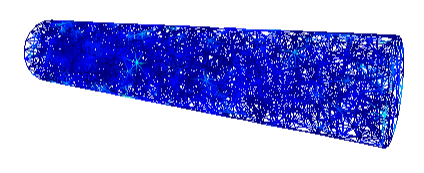
\includegraphics[width=0.5\textwidth]{wireframe}
  \caption{ Wireframe rendering of cylindrical domain. The colors are handled similarly to in Figure \ref{surface}. }
  \label{wireframe}
\end{figure}

\begin{figure}[!ht]
  \centering
    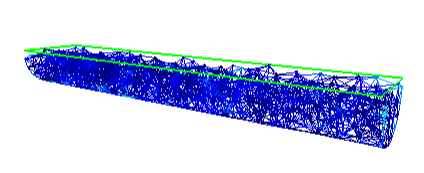
\includegraphics[width=0.5\textwidth]{clipy}
  \caption{ Wireframe rendering of cylindrical domain clipped in the Y direction. }
  \label{clipy}
\end{figure}

\subsection{Volume Rendering}

The final rendering StochSS offers is a volume rendering (Figure \ref{volume}). It uses a basic ray-tracing implementation following the one in \cite{congote}.

\begin{figure}[!ht]
  \centering
    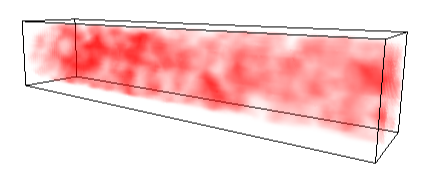
\includegraphics[width=0.5\textwidth]{volume}
  \caption{ This is the volume rendering of the same data shown above. The idea behind volume rendering is to color darkly areas with high concentrations and leave volumes with low concentrations transparent. The transparency makes it possible to see inside a volume rendering, and so the slicing as shown in the surface and wireframe renderings is not used. }
  \label{ volume }
\end{figure}

